% Document template for ANS Journals
% Options: footnoteAtEnd - Places all footnotes at the end of document
%               Usage: \documentclass[footnoteAtEnd]{style/nseJournal}
\documentclass{nseJournal}
\usepackage{local}
\usepackage{algorithm}
\usepackage{algorithmic}
\usepackage{caption}

\begin{document}

\title{Krylov Linear Solvers and Quasi Monte Carlo Methods for Transport Simulations}

% Use the \addAuthor macro to add authors in the order they should appear. The second argument corresponds to
% the affiliation declared below.
\addAuthor{Sam Pasmann}{a}
\addAuthor{C. T. Kelley}{b}
\addAuthor{\correspondingAuthor{Ryan McClarren}}{a}
\correspondingEmail{rmcclarr@nd.edu}

% Affiliations can be added in the order they should appear. For breaks in addresses, use either \\ or \tabularnewline
\addAffiliation{a}{Department of Aerospace and Mechanical Engineering\\ University of Notre Dame\\ Fitzpatrick Hall, Notre Dame, IN 46556}
\addAffiliation{b}{North Carolina State University, Department of
Mathematics\\ 3234 SAS Hall, Box 8205\\ Raleigh NC 27695-8205}

% Add keywords to appear in Abstract in the order they should appear
\addKeyword{Quasi Monte Carlo Methods}
\addKeyword{Krylov Linear Solvers}

\titlePage

\begin{abstract}

\end{abstract}

\section{Introduction}
\label{sec:intro}


\section{Methods}
\label{sec:methods}


 %%%%%%%%%%%%%%%%%%%%%%%%%%%%%%%%%%%%%%%%%%%%%%%%%%%%%%%%%%%%%%%%%%
 %%%%%%%%%%%%%%%%%%%%%%%%%%%%%%%%%%%%%%%%%%%%%%%%%%%%%%%%%%%%%%%%%%

\subsection{Source Iteration}
Source iteration is Picard iteration for the fixed point problem. We begin with an initial guess $\phi_0$ and solve Equation \ref{eq:transport} for $\psi_1$. Given that:

\begin{equation}
	\label{eq:phi}
	\phi_n = \int_{-1}^{1}\psi_n d\mu .
\end{equation}

That is, given $\phi_n$ compute $\psi_{n+1}$, then compute $\phi_{n+1}$ given Equation \ref{eq:phi} until convergence where $\phi_{n+1} = \phi_{n}$. Given this iterative scheme, Equation \ref{eq:transport} and Equation \ref{eq:phi} combine to become:

\begin{equation}\label{equation:SI}
    \mu\frac{\partial\psi_{n+1}}{\partial x}(x,\mu)+ \Sigma_t(x)\psi_{n+1}(x,\mu) = \frac{1}{2} \left[ \Sigma_s(x)\phi_{n}(x) + q(x)\right].
\end{equation}

Given an angular discretization, this becomes a linear system of equations which, can be represented in operator notation where:
\[
	\phi = \cals(\phi, q, \psi_l, \psi_r)
\]
and
\[
	\calk(\phi) = \cals(\phi, 0, 0, 0) \mbox{ and }
	f = \cals(0, q, \psi_l, \psi_r).
\]
Where Source Iteration is represented as
\[
	\phi_{n+1} = \calk(\phi_n) + f,
\]
to get
\[
	A \phi \equiv (I - \calk) \phi = f
\]
which we can send to a linear solver. It is important to note that the methods employed ensure that we never form the matrix $A$.  Instead, the Monte Carlo simulation will compute the action of matrix $A$ on $\phi$.

 %%%%%%%%%%%%%%%%%%%%%%%%%%%%%%%%%%%%%%%%%%%%%%%%%%%%%%%%%%%%%%%%%%
 %%%%%%%%%%%%%%%%%%%%%%%%%%%%%%%%%%%%%%%%%%%%%%%%%%%%%%%%%%%%%%%%%%

%\subsection{The Matrix-Vector Product}

 
 %%%%%%%%%%%%%%%%%%%%%%%%%%%%%%%%%%%%%%%%%%%%%%%%%%%%%%%%%%%%%%%%%%
 %%%%%%%%%%%%%%%%%%%%%%%%%%%%%%%%%%%%%%%%%%%%%%%%%%%%%%%%%%%%%%%%%%

\subsection{Krylov Subspace Methods}

An order-$r$ Krylov subspace is defined with notation from the previous section as:
\begin{equation}
K_r = \textrm{span}(\phi, A\phi, A^{2}\phi, ..., A^{r-1}\phi).
\end{equation}

For each experiment, two Krylov methods \cite{ctk:roots}, GMRES \cite{gmres} and Bi-CGSTAB \cite{bicgstab}, were used. The Generalized Minimum RESidual (GMRES) is one of the most common Krylov methods. When solving $A\vec{\phi}=\vec{f}$, GMRES minimized $||f-A\phi||_2$ over the $k^{th}$ Krylov subspace. For every iteration, the GMRES stores an additional Krylov vector. For problems that require many iterations this may lead to memory constraints. Bi-CGSTAB is a low-storage Krylov method that is memory bounded throughout the algorithm. However, the memory savings come from information that is thrown out with each iteration and therefore Bi-CSTAB will generally require more iterations to converge than GMRES. Nonetheless, as we will in section \ref{sec:results}, both Krylov methods will require far fewer iterations than the standard SI. 


 %%%%%%%%%%%%%%%%%%%%%%%%%%%%%%%%%%%%%%%%%%%%%%%%%%%%%%%%%%%%%%%%%%
 %%%%%%%%%%%%%%%%%%%%%%%%%%%%%%%%%%%%%%%%%%%%%%%%%%%%%%%%%%%%%%%%%%

\subsection{Monte Carlo Sweep}

Monte Carlo methods use the central limit theorem and the law of large numbers to solve integral equations by randomly sampling the probability space and approximating the theoretical expected value \cite{Lux1991, Murray1977}. Monte Carlo for neutron transport seeks to simulate the behavior of many particles from \textit{birth} to \textit{death} and gain an approximate description of the system. Physics equations and cross section data are used to model collisions while quantities of interest, like scalar flux ($\phi$), are tallied in the appropriate spatial region. Standard Monte Carlo techniques have been shown to converge at a rate of $O(N^{-0.5})$, where $N$ is the number of particles, regardless of the dimensionality of the problem \cite{Brown2005, Brown2006, Brown2016}. 

In a MC simulation with scattering, each particle path represents a Markovian process or \textit{random walk} and the resulting algorithm is one that is massively parallel \cite{Carter1975, Kroese2011, willert2012hybrid}. Due to the noise inherent from random sampling, high-performance Monte Carlo codes often rely on simulating large numbers of particles across many nodes \cite{Pereira2013}. Nonetheless, the computational costs remain high and many variance reduction techniques have been developed to improve convergence properties \cite{McClarren2018}.



\subsubsection{Quasi-Monte Carlo}

One such variance reduction method is the use of Quasi-Monte Carlo (QMC). QMC  uses quasi-random low-discrepancy sequences in place of pseudo-random number generators in MC simulations. Low-discrepancy sequences use deterministic algorithms to sample the phase space in \textit{self-avoiding}  manner thereby approaching a more uniform distribution and approximating the expectation more efficiently. This results in a theoretical convergence rate of $O(N^{-1})$ compared to the $O(N^{-0.5})$ from pseudo-randomly placed points \cite{Palluotto2019}.  Because the low-discrepancy sequences sample the phases-space in a deterministic manner they introduce a dependence, albeit a weak one, on the dimensionality of the problem \cite{Hickernell2002}. Commonly used low-discrepancy sequences include the Halton Sequence and Sobol Sequence \cite{Niederreiter1992}. For low-dimensional problems, the Halton sequence has been shown to provide the best results. However, for higher-dimensional problems the Sobol Sequence is most commonly used.

QMC is commonly used in Finance to evaluate high-dimensional integrals \cite{Dagpunar2007} and there has also been recent work in using QMC in radiative heat transfer applications \cite{MOROKOFF1993, Palluotto2019}. However, QMC has largely been ignored by the particle transport community \cite{Spanier1995}. This is because the deterministic nature of the low discrepancy sequence breaks the Markovian assumption needed for the particle \textit{random walk}. Therefore QMC must be implemented in specific applications which are not Markovian processes, such as the initial starting position of each particle, or steps must be take to ensure the Markovian assumption is held. Presently, there have been two separate strategies for implementing QMC in particle transport while maintaining the Markovian assumption. The first is known generally as randomized-QMC or (RQMC) which includes a host of strategies that attempt to reorder the sequence so each point is individually uniformly distributed within the space but the collective still retain their low-discrepency. \cite{Fox1999, Spanier1995, Farmer2020, MOROKOFF1993, Konzen2019}. The second, makes use of the previously discussed  deterministic and iterative methods in which the problem can be modeled in the Monte Carlo simulation as a purely absorbing problem and the scattering term is iterated upon using one of the previously discussed methods removing the need for a \textit{random walk} process \cite{Pasmann2021}.

\begin{figure}[h]
\centerline{
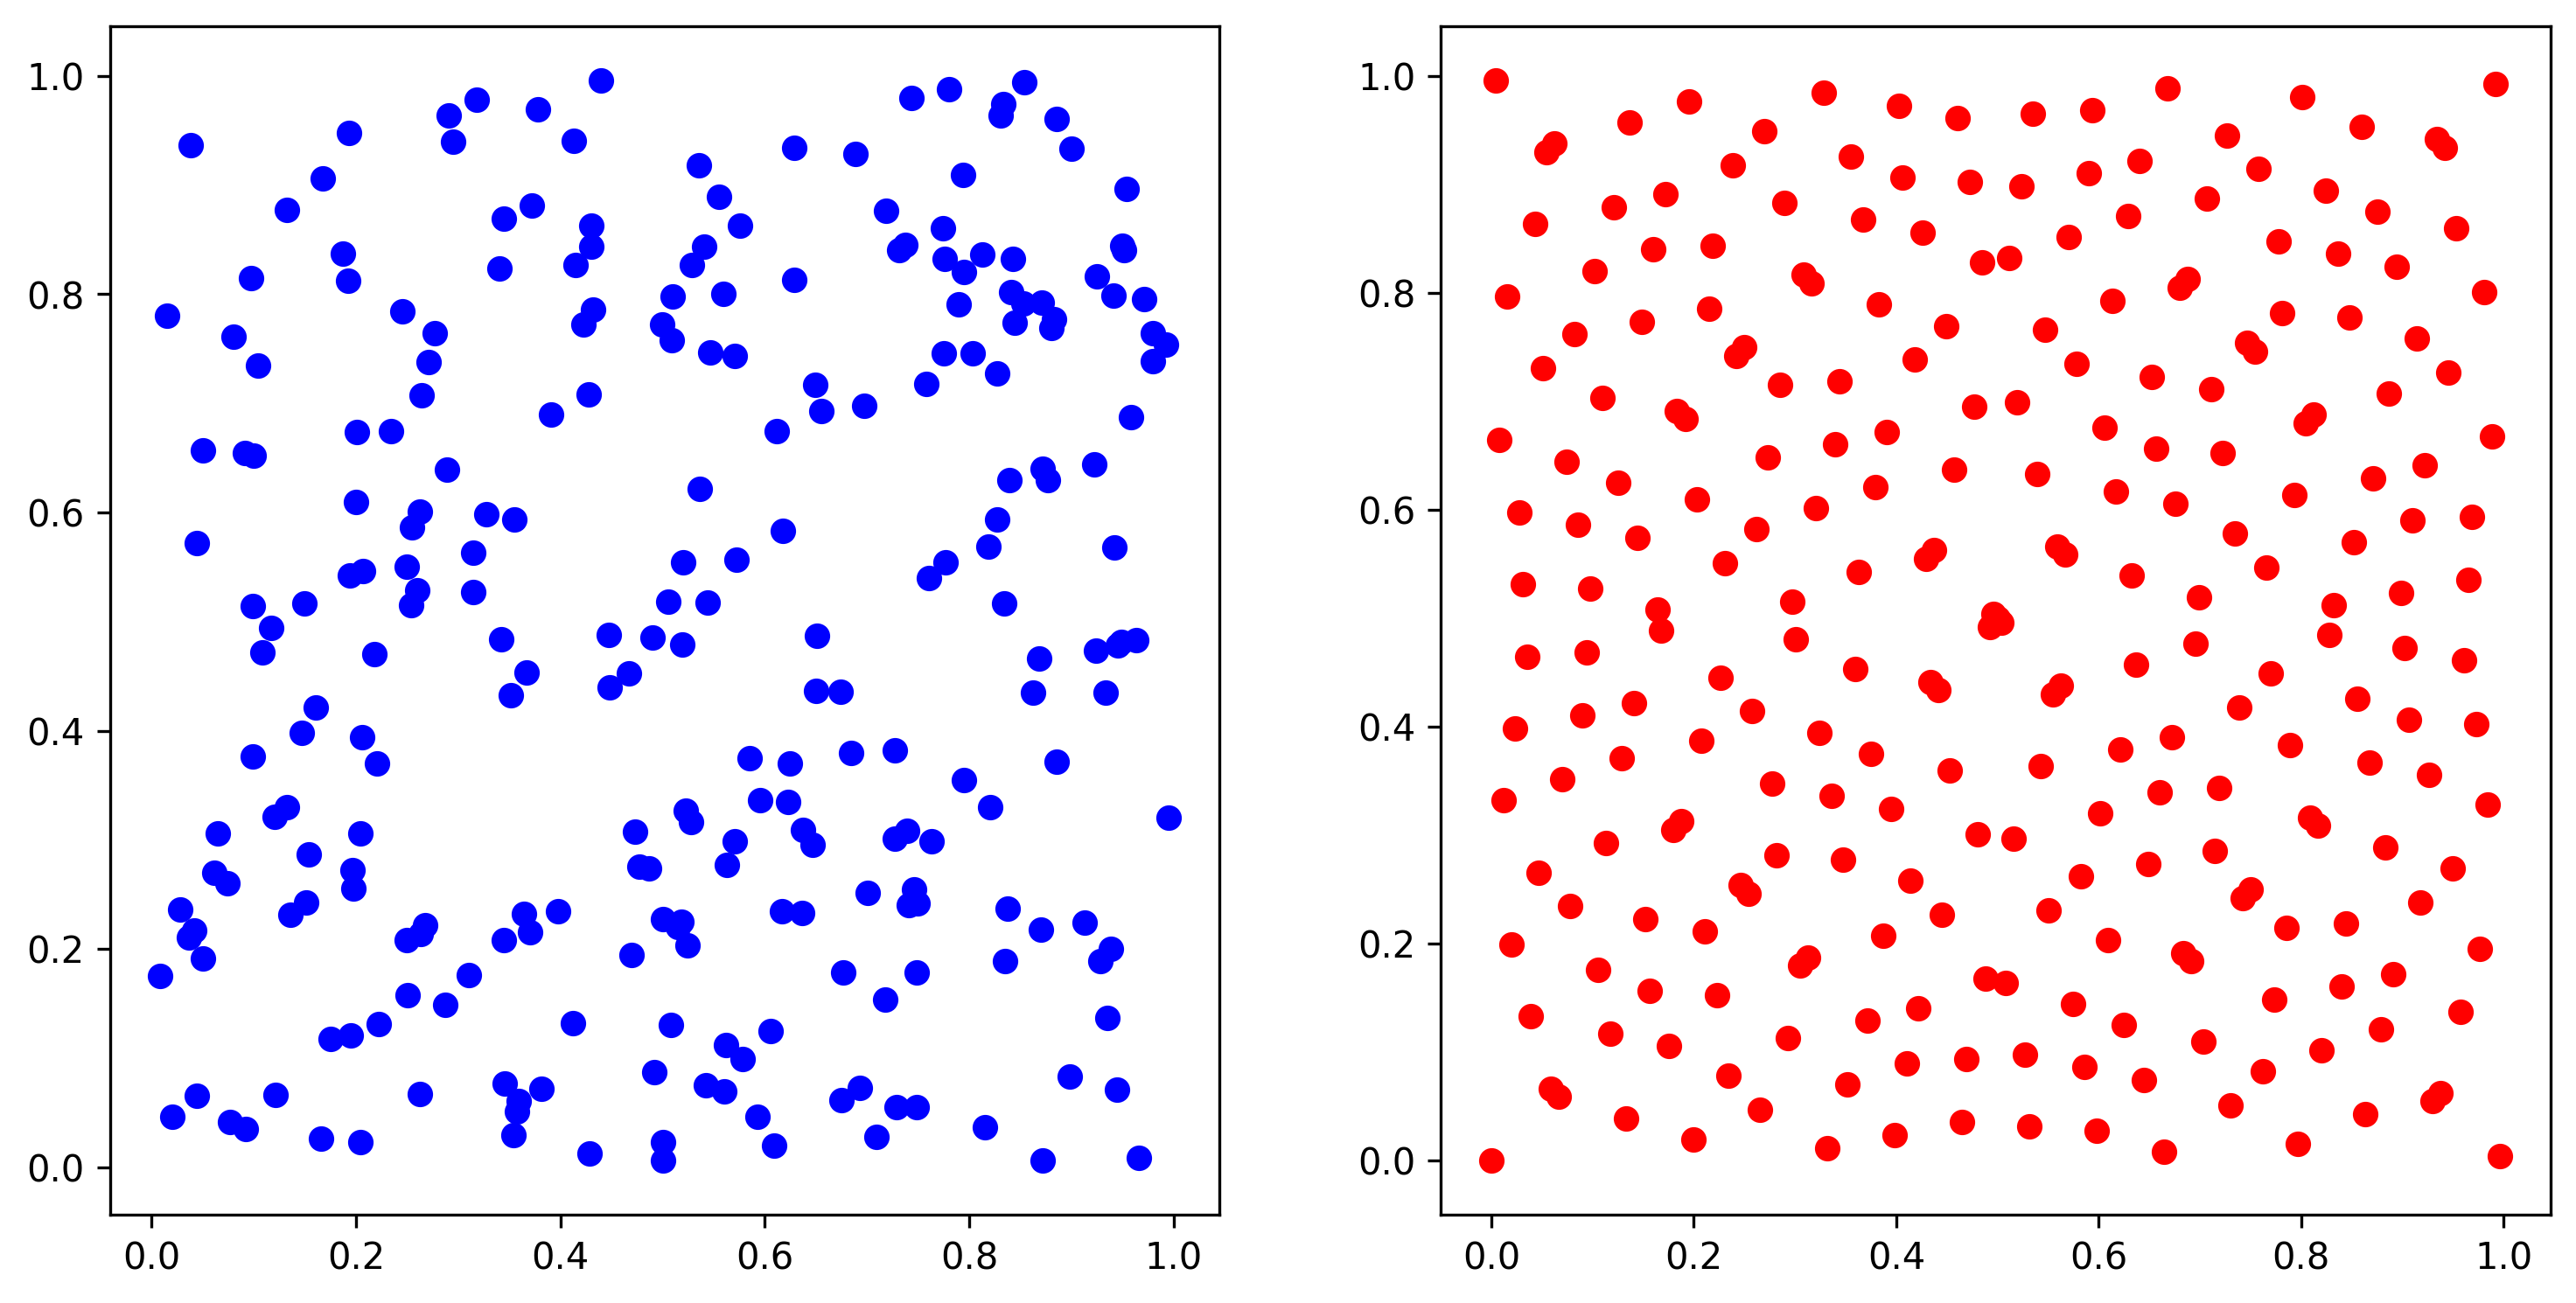
\includegraphics[width=3.5in]{FIGURES/sobol.png}
}
\caption{\label{fig:sobol} 256 points generated in a unit square with pseudo random points (left) and the Sobol sequence (right).}
\end{figure}


\subsubsection{Multigroup Equations}

In general geometry, the multigroup equations for $G$ groups are:
\begin{equation}\label{eq:MG}
\mu  \frac{\partial \psi_g}{\partial x} (x,\mu) + \Sigma_{t,g}(x) \psi_g(x,\mu) =
\frac{1}{2} \sum_{g'=1}^G \Sigma_{s,g'\rightarrow g}(x) \int_{-1}^1 \psi_{g'}(x, \mu') \dmup + \frac{q_g(x)}{2} \quad g=1,\dots,G.
\end{equation}The boundary conditions become:
\[
\psi_g(0, \mu) = \psi_{l,g}(\mu), \mu > 0; \psi_g(\tau, \mu) = \psi_{r,g}(\mu),
\mu < 0.
\]

In matrix form, these equations are
\begin{equation}\label{eq:MGmat}
\mu  \frac{\partial \vec{\psi}}{\partial x} (x,\mu) + \underline{\Sigma}_{t}(x) \vec{\psi}(x,\mu) =
\frac{1}{2}  \underline{\Sigma}_{s}(x) \int_{-1}^1 \vec{\psi}(x, \mu') \dmup + \frac{\vec{q}(x)}{2},
\end{equation}
where
\begin{equation}\label{eq:vecs}
\vec{\psi} = (\psi_1, \psi_2, \dots, \psi_G)^\mathrm{T}, \qquad \vec{q} = (q_1, q_2, \dots, q_G)^\mathrm{T}, 
\end{equation}
\begin{equation}\label{eq:MatricesT}
 \underline{\Sigma}_{t}(x)  = \begin{pmatrix} \Sigma_{t,1}(x) & 0 & \dots\\
 0 & \Sigma_{t,2}(x) & 0 \dots \\
 \vdots & & \ddots\\ 
 0 & \dots & 0 & \Sigma_{t,G}(x) 
 \end{pmatrix}, 
\end{equation}
and
\begin{equation}\label{eq:MatricesS}
 \underline{\Sigma}_{s}(x)  = \begin{pmatrix} \Sigma_{s,1\rightarrow 1}(x) & \Sigma_{s,2\rightarrow 1}(x)  & \dots & \Sigma_{s,G\rightarrow 1}(x) \\
 \Sigma_{s,2\rightarrow 1}(x) & \Sigma_{s,2\rightarrow 1}(x)  & \dots & \Sigma_{s,G\rightarrow 2}(x) \\
 \vdots & \vdots & & \vdots\\
 \Sigma_{s,G\rightarrow 1}(x) & \Sigma_{s,G\rightarrow 1}(x)  & \dots & \Sigma_{s,G\rightarrow G}(x) \\
 \end{pmatrix},.
\end{equation}


\section{Algorithm}
\label{sec:algorithm}




 %%%%%%%%%%%%%%%%%%%%%%%%%%%%%%%%%%%%%%%%%%%%%%%%%%%%%%%%%%%%%%%%%%
 %%%%%%%%%%%%%%%%%%%%%%%%%%%%%%%%%%%%%%%%%%%%%%%%%%%%%%%%%%%%%%%%%%
The program was written in Julia, a scientific computing language that combines the compiler capabilities of C++ and the syntax of Matlab and Python. The code and primary documentation are available here \href{https://github.com/ctkelley/Krylov_QMC} {Krylov\textunderscore QMC} \cite{ctk:krylovqmc}. The linear and nonlinear solvers come from the Julia package \href{https://github.com/ctkelley/SIAMFANLEquations.jl}{SIAMFANLEQ.jl} \cite{ctk:siamfanl}. The documentation for these codes is in the \href{https://github.com/ctkelley NotebookSIAMFANL}{Juila notebooks} \cite{ctk:notebooknl} and the book \cite{ctk:fajulia} that accompany the package. 

\noindent\begin{minipage}{\textwidth}
\begin{minipage}{0.45\textwidth}
		\centering
		\captionof{algorithm}{Source Iteration}
		\label{alg:SI}
		\begin{algorithmic}[1]
		\STATE Initialize $\phi_0$
		\WHILE{($r>\textrm{tolerance}$)}
			\STATE $q = \phi_{n-1}*\Sigma_{s} + \textrm{source}$
			\STATE $\phi_n = \mbox{QMC Sweep}(q)$
			\STATE $r_{i} = \frac{||\phi_n - \phi_{n-1}||}{||\phi_{n-1}||}$
		\ENDWHILE
		\STATE Return: $\phi$
	\end{algorithmic} 
\end{minipage}
\hfill
\begin{minipage}{0.45\textwidth}
	\centering
	\captionof{algorithm}{QMC Sweep $(q)$}
	 \label{alg:qmc_sweep}
	\begin{algorithmic}[1]
		\STATE Initialize Low-Discrepancy-Sequence
		\FOR {$i$ in $N$}
			\STATE Assign $r_i$ and $\mu_i$
			\FOR {$j$ in Zones}
				\STATE Move particle across $\textrm{Zone}_j$
				\STATE Tally($r, \mu, weight$)
			\ENDFOR
		\ENDFOR
		\STATE Return: $\phi$
	\end{algorithmic} 
\end{minipage}
\end{minipage}





\section{Computational Results}
\label{sec:results}
In this section we consider an example from
\cite{cesinh}. The formulation of the transport
problem is taken from \cite{ctk:jeff1}. The equation for the angular
flux \(\psi\) is

\[
\mu \frac{\partial \psi}{\partial x} (x,\mu) + \Sigma_t(x) \psi(x,\mu) =
\frac{1}{2} \left[ \Sigma_s(x) \int_{-1}^1 \psi(x, \mu') \dmup + q(x) \right]
 \mbox{ for } 0 \le x \le \tau
\]

The boundary conditions are

\[
\psi(0, \mu) = \psi_l(\mu), \mu > 0; \psi(\tau, \mu) = \psi_r(\mu),
\mu < 0.
\]

The notation is

\begin{itemize}
\item
  \(\psi\) is intensity of radiation or angular flux at point \(x\) at
  angle \(\cos^{-1} (\mu)\)
\item
  \(\phi = \phi(x) = \int_{-1}^{1}\psi(x,\mu) \ d\mu\) is the scalar
  flux, the \(0^{th}\) angular moment of the angular flux. -
  \(\tau < \infty\), length of the spatial domain. -
  \(\Sigma_s \in C([0,\tau])\) is the scattering cross section at \(x\)
  - \(\Sigma_t \in C([0,\tau])\) is the total cross section at \(x\) -
  \(\psi_l\) and \(\psi_r\) are incoming intensities at the bounds -
  \(q \in C([0,\tau])\) is the fixed source
\end{itemize}


\subsection{The Garcia-Siewert Example}
\label{the-garcia-siewert-example}

In this example \[
\tau=5, \Sigma_s(x) =\omega_0 e^{-x/s},  \Sigma_t(x) = 1, q(x) = 0, \psi_l(\mu) = 1, \psi_r(\mu) = 0.
\]

\subsection{Solvers}
\label{subsec:solvers}

The linear and nonlinear solvers come from the Julia package
\href{https://github.com/ctkelley/SIAMFANLEquations.jl}{SIAMFANLEQ.jl}
\cite{ctk:siamfanl}. The documentation for these codes is in the
\href{https://github.com/ctkelley/NotebookSIAMFANL}{Juila notebooks}
that accompany the package \cite{ctk:notebooknl}. 
These are part of a book project \cite{ctk:fajulia}. 

\subsection{Source Iteration and Krylov Methods}
\label{source-iteration-and-krylov-methods}

We use two krylov methods \cite{ctk:roots}, GMRES \cite{gmres} and
Bi-CGSTAB \cite{bicgstab}.

\subsection{QMC}\label{qmc}

\subsection{Validation and calibration study}
\label{validation-and-calibration-study}

I'll compare the results from the SN computation to what I get from
Sam's QMC code. My SN results are for a very fine spatial mesh and fine
enough angular mesh. They are good to at least six figures and I will
regard them as exact for this study.

I will use the SN results for the table in the Garcia-Siewert paper and
get results from QMC in the following way

\begin{itemize}
\item
  For a give N and Nx I will get cell average fluxes from Sam's code.
\item
  I will use the same code to generate the tables that I used for the SN
  fluxes. That code is \textbf{src/sn\_tabulate.jl}
\item
  I will take the two 11 x 2 arrays of results DataSN and DataQMC and
  compoute componentwise relative error with
\end{itemize}

\begin{verbatim}
Derr = (DataSN-DataQMC)./DataSN
\end{verbatim}

\subsection{QMC and Krylov Linear Solvers}
\label{qmc-and-krylov-linear-solvers}

I can solve the QMC linear problem with both Krylov methods now and,
just like the classical case, I'm seeing fewer than half of the number
of transport sweeps. Herewith the results for N=1000 and Nx= 100.







\clearpage


\section{Conclusion}
\label{sec:conclusion}


\pagebreak
\section*{Acknowledgments}


This work was funded by the Center for Exascale Monte-Carlo Neutron Transport (CEMeNT) a PSAAP-III project funded by the Department of Energy, DE-NA003967, 
%
and supported by National Science Foundation Grants
% RTG
DMS-1745654,
and
% New NSF
DMS-1906446.


\pagebreak
\bibliographystyle{ans_js}    %custom ANS journal submission template bibliography style
\bibliography{qmckrylov}

\end{document}


